\chapter{Appendix I: List of Datasets}
\label{chap:datasets_app}
\setcounter{table}{0}
\renewcommand{\thetable}{A\arabic{table}}

\begin{table}[ht]
\caption{Descriptions and names of the datasets used.}
    \centering
    \begin{tabular}{>{\raggedright\arraybackslash}p{0.3\linewidth} | >{\raggedright\arraybackslash}p{0.3\linewidth} | >{\raggedright\arraybackslash}p{0.3\linewidth}} 
        \toprule
        Official name              & Description            & Alternative names  \\
        \midrule
        Annual Metropolitan and Regional Train Origin-Destination Counts  & O-D data provided from the DTP with hourly counts of O-D trips with total patronage and average daily patronage.  &  
        Original O-D data /
        Unprocessed O-D data \\ \hline
        Processed Annual Metropolitan and Regional Train Origin-Destination Counts          & Processed O-D data aggregated to 15 minute periods as described in \refandname{subsec:data_recon}.&  
        Input O-D data /
        Processed O-D data
          \\ \hline
        Train Service Passenger Counts   & Boardings, alightings and arrival and departure loads of train services rounded to the nearest 10 passengers. & 
        Historical boardings / 
        Boardings /
        Passenger counts
        \\ 
        \bottomrule
 GTFS& A GTFS feed from Sept 9th- 15th was used as this period reflected a normal timetable without any modifications for planned works & General Transit Feed Specification\\ \hline
 WoB Counts Output& Number of agents on services between adjacent stations. &Agent counts / Counts\\ \hline
 WoB Journeys Output& The number of agents taking a particular journey itinerary. &Journeys\\ \hline
 WoB Journey Legs Output& The detailed itinerary of agent journeys. &Journey legs / Journey itinerary\\ \hline
 WoB Transfers Output & The transfer details for agents making journeys involving transfers, including the transfer station and service details. & Transfers\\
    \end{tabular}
    \label{tab:datasets}
\end{table}

\chapter{Appendix II: Crowding Validation Results}
\label{chap:crowding_results_app}

\begin{figure}[h]
    \centering
    \begin{subfigure}{0.45\linewidth}
        \centering
        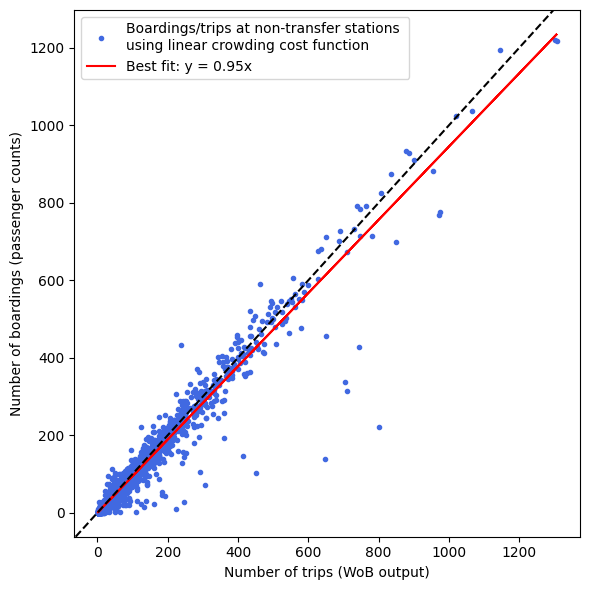
\includegraphics[width=\linewidth]{images/Validation/val_lin.png}
        \label{fig:val_lin}
    \end{subfigure}
    \hfill
    \begin{subfigure}{0.45\linewidth}
        \centering
        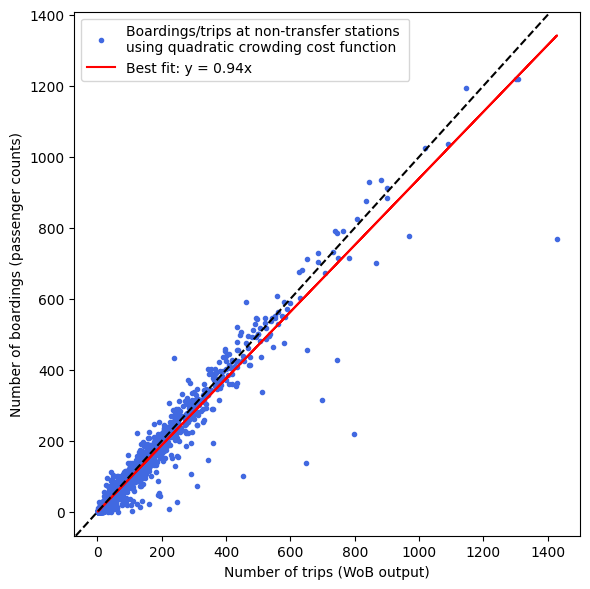
\includegraphics[width=\linewidth]{images/Validation/val_quad.png}
        \label{fig:val_quad}
    \end{subfigure}
    \vskip\baselineskip
    \begin{subfigure}{0.45\linewidth}
        \centering
        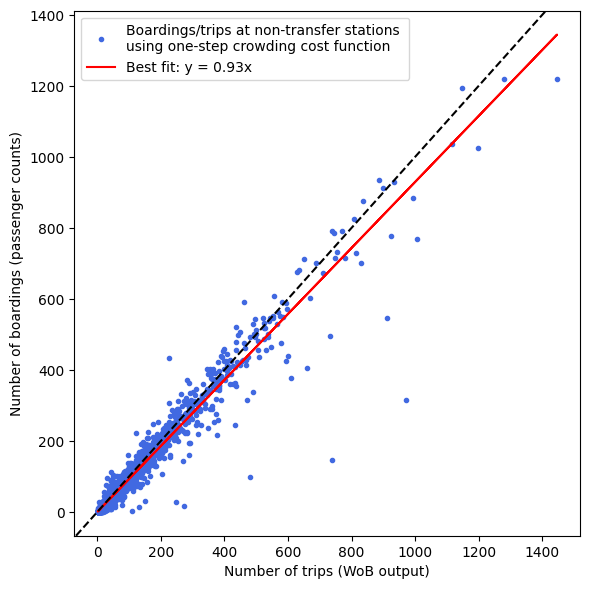
\includegraphics[width=\linewidth]{images/Validation/val_one.png}
        \label{fig:val_one}
    \end{subfigure}
    \hfill
    \begin{subfigure}{0.45\linewidth}
        \centering
        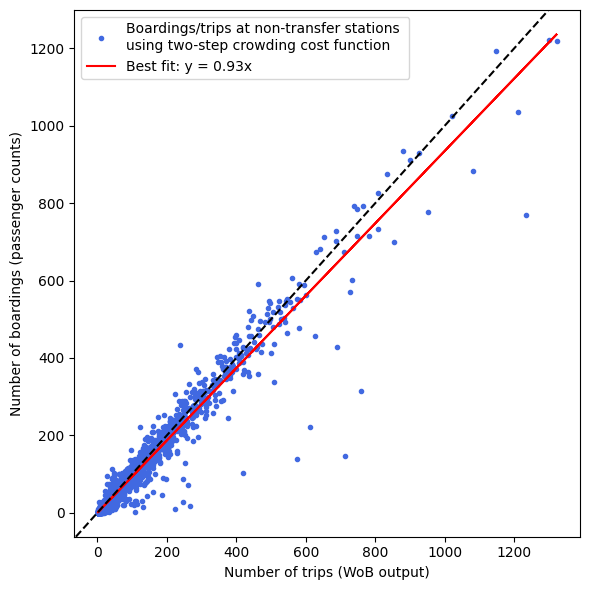
\includegraphics[width=\linewidth]{images/Validation/val_two.png}
        \label{fig:val_two}
    \end{subfigure}
    \caption[Full plots of the comparison between passenger counts data and WoB journey output using various crowding cost functions]{Comparison between passenger counts data and WoB journey output using the various crowding cost functions at non-transfer stations with a linear line of best fit. From left to right and top to bottom, the crowding cost functions used are linear, quadratic, one-step and two-step models. The default parameters were used, $a_0=0.25, a_1=0.5, a=5, b=1, c=0.01$.}
    \label{fig:validation_grid}
\end{figure}



\begin{table}[t]
\centering
\caption{Results from fitting model outputs with the two-step crowding cost function.}
    \csvautotabular{data/two_step_results.csv}
\end{table}

\begin{table}[t]
\centering
\caption{Results from fitting model outputs with the one-step crowding cost function.}
    \csvautotabular{data/one_step_results.csv}
\end{table}


\chapter{Appendix III: Case Study}
\label{chap:case_study_app}

\begin{figure}[ht]
    \centering
    \includesvg[width=0.75\columnwidth]{images/Case_Study/Introduction/Victorian-Train-Network-Map-May-2023-v3.pdf.svg}
    \caption[Map of Melbourne's rail network]{A map of the rail network system across Melbourne, as well as the state of Victoria. The lines in purple are regional rail and coach V/Line services, and the grey dotted line is the upcoming Metro Tunnel expansion. The regional and upcoming lines were not included in this investigation.}
    \label{fig:melb-network-map}
\end{figure}

\subsubsection{Further Rollingstock Information}
Rail operator Metro Trains Melbourne runs a fleet of over 400 1500V DC4 EMU (electric multiple unit) trains over almost 1,000 kilometres of broad gauge (1600mm) track. The fleet consists of a variety of trains: Commonwealth Engineering Trains (EDI Rail or Alstom refurbishment), the X’Trapolis 100, Siemens Nexus and most recently, the HCMT (High Capacity Metro Train). Unlike the other two set 3-car EMUs, the HCMT has greater carrying capacity, consisting of seven cars with open configuration, enabling passengers to walk the entire length of the train unimpeded. 

\begin{table}[ht]
    \centering
      \caption{Assignment of train lines to City Loop station platforms}
    \begin{tabular}{c|l}
         Platform 1& Hurstbridge and Mernda \\
         Platform 2& Pakenham and Cranbourne\\
         Platform 3& Sunbury, Craigieburn and Upfield\\
         Platform 4& Belgrave, Lilydale, Alamein and Glen Waverley\\
    \end{tabular}

    \label{tab:cityloop_platforms}
\end{table}

\begin{figure}[ht]
    \centering
    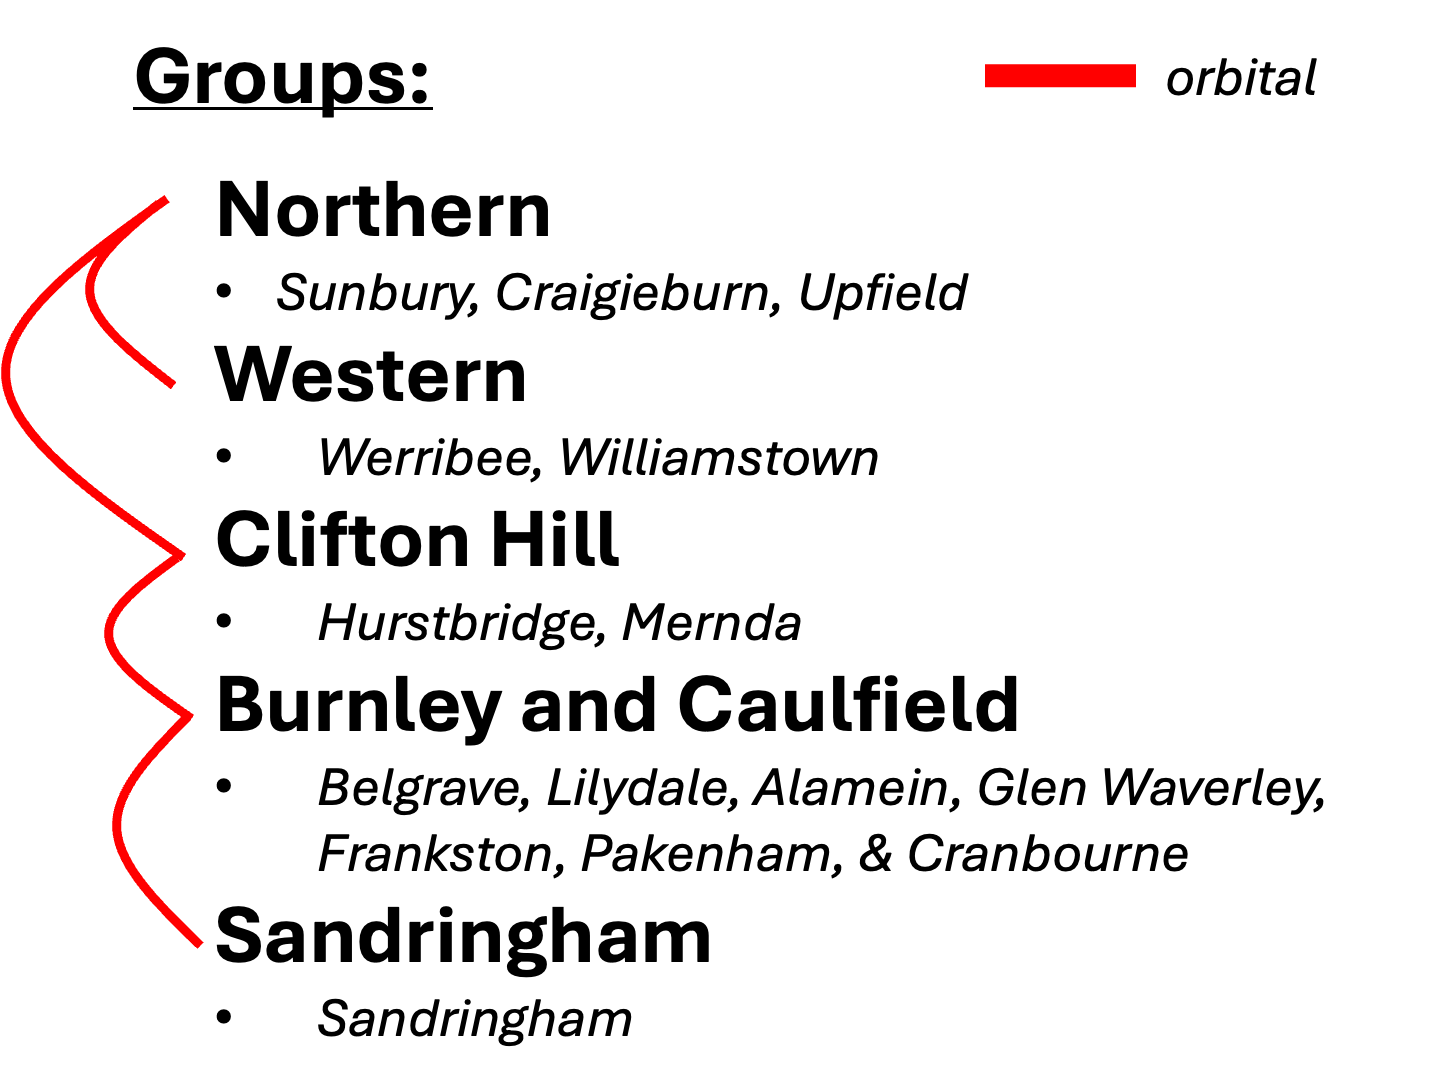
\includegraphics[width=0.75\linewidth]{images/Case_Study/Appendix/orbitalgroupsss.png}
    \caption[Specification of train line relationships]{Specification of line relationships, where lines drawn in red, or within same group are specified as orbital. The remaining relations, where the start or end of journey is not in city are specified as cross-city}
    \label{fig:enter-label}
\end{figure}